% What We Signed Up For -- the Final SoW, seeds, and what Neotix asked of us
% Build: latexmk -pdf sow_and_seeds_guide.tex && latexmk -c   (all figures are TikZ; no external files)
\documentclass[11pt,a4paper]{article}

\usepackage[margin=2.1cm,headheight=14pt]{geometry}
\usepackage{lmodern}
\usepackage[T1]{fontenc}
\usepackage{microtype}
\usepackage{xcolor}
\usepackage{amsmath}
\usepackage{amssymb}
\usepackage{tikz}
\usetikzlibrary{arrows.meta,positioning,shapes.geometric,shapes.misc,fit,backgrounds,calc,patterns,decorations.pathreplacing}
\usepackage[most]{tcolorbox}
\usepackage{booktabs}
\usepackage{tabularx}
\usepackage{array}
\usepackage{enumitem}
\usepackage{fontawesome5}
\usepackage{fancyhdr}
\usepackage{titlesec}
\usepackage{float}
\usepackage{needspace}
\usepackage{caption}
\usepackage[hidelinks]{hyperref}

% ---------------------------------------------------------------- colours (as the other guides)
\definecolor{ink}{HTML}{1F2933}
\definecolor{sky}{HTML}{2B6CB0}
\definecolor{skylight}{HTML}{EBF4FF}
\definecolor{leaf}{HTML}{2F855A}
\definecolor{leaflight}{HTML}{E6FFFA}
\definecolor{sun}{HTML}{B7791F}
\definecolor{sunlight}{HTML}{FFFAEB}
\definecolor{rose}{HTML}{C53030}
\definecolor{roselight}{HTML}{FFF5F5}
\definecolor{grape}{HTML}{6B46C1}
\definecolor{grapelight}{HTML}{F3EEFF}
\definecolor{stone}{HTML}{718096}
\definecolor{stonelight}{HTML}{F4F6F8}

\color{ink}
\hypersetup{colorlinks=true,linkcolor=sky,urlcolor=sky}
\captionsetup{font=small,labelfont={bf,color=sky}}

\titleformat{\section}{\Large\bfseries\color{sky}}{\thesection}{0.8em}{}[{\color{sky!40}\titlerule[1pt]}]
\titleformat{\subsection}{\large\bfseries\color{ink}}{\thesubsection}{0.7em}{}
\pagestyle{fancy}
\fancyhf{}
\fancyhead[L]{\small\color{stone}\faFileSignature\ \ What We Signed Up For}
\fancyhead[R]{\small\color{stone}Final SoW, seeds and client asks}
\fancyfoot[C]{\small\color{stone}\thepage}
\renewcommand{\headrulewidth}{0.4pt}
\setlist{itemsep=2pt,topsep=4pt}
\newcommand{\sectionbreak}{\needspace{20\baselineskip}}
\newcommand{\subsectionbreak}{\needspace{14\baselineskip}}

\newtcolorbox{eli5}{enhanced,before upper={\raggedright},colback=sunlight,colframe=sun,boxrule=0.8pt,arc=3mm,
  title={\faChild\ \ In plain words},fonttitle=\bfseries,coltitle=white}
\newtcolorbox{incode}{enhanced,before upper={\raggedright},colback=leaflight,colframe=leaf,boxrule=0.8pt,arc=3mm,
  title={\faCode\ \ In the code},fonttitle=\bfseries}
\newtcolorbox{careful}[1][Careful]{enhanced,before upper={\raggedright},colback=roselight,colframe=rose,boxrule=0.8pt,arc=3mm,
  title={\faExclamationTriangle\ \ #1},fonttitle=\bfseries}
\newtcolorbox{keyidea}{enhanced,before upper={\raggedright},colback=skylight,colframe=sky,boxrule=0.8pt,arc=3mm,
  title={\faLightbulb\ \ Key idea},fonttitle=\bfseries}
\newtcolorbox{quotebox}[1]{enhanced,before upper={\raggedright\itshape},colback=grapelight,colframe=grape,boxrule=0.8pt,arc=3mm,
  title={\faQuoteLeft\ \ #1},fonttitle=\bfseries}
% A numbered "ask" card for Birhanu's requests.
\newtcolorbox{ask}[2]{enhanced,before upper={\raggedright},colback=white,colframe=grape,boxrule=0.8pt,arc=2mm,
  left=8pt,attach boxed title to top left={xshift=4mm,yshift=-2mm},boxed title style={colback=grape,arc=1mm},
  title={\bfseries Ask #1: #2},fonttitle=\small\color{white}}

% Small coloured chips used in tables.
\newcommand{\chip}[2]{\tikz[baseline=(chipnode.base)]\node[fill=#1,text=white,rounded corners=2pt,inner sep=2pt,font=\scriptsize\bfseries](chipnode){#2};}
\newcommand{\yes}{\textcolor{leaf}{\faCheck}}
\newcommand{\no}{\textcolor{rose}{\faTimes}}
\newcommand{\tool}[1]{\texttt{\small #1}}

\tikzset{
  box/.style={draw=#1,fill=#1!8,rounded corners=3pt,thick,align=center,inner sep=5pt,font=\small},
  box/.default=sky,
  arr/.style={-{Latex[length=2.4mm]},thick,draw=stone},
  lbl/.style={font=\scriptsize,text=stone,align=center},
}

\begin{document}

% ====================================================================== title
\begin{tikzpicture}[remember picture,overlay]
  \fill[sky] (current page.north west) rectangle ([yshift=-4.3cm]current page.north east);
  \node[anchor=north west,text=white,font=\fontsize{26}{30}\selectfont\bfseries] at ([xshift=2.1cm,yshift=-1.25cm]current page.north west) {What We Signed Up For};
  \node[anchor=north west,text=white!85!sky,font=\large] at ([xshift=2.1cm,yshift=-2.45cm]current page.north west)
    {The Final Statement of Work, how seeds make the evaluation fair, and what Neotix asked of us};
  \node[anchor=north west,text=white!75!sky,font=\small] at ([xshift=2.1cm,yshift=-3.3cm]current page.north west)
    {Neotix Robotics-Team \textbullet\ for the team \textbullet\ 26 Nov 2026 \textbullet\ from the signed SoW and the e-mail thread (16--23 Nov)};
\end{tikzpicture}
\vspace*{3.1cm}
\thispagestyle{empty}

\section*{The whole thing on one page}

\begin{center}
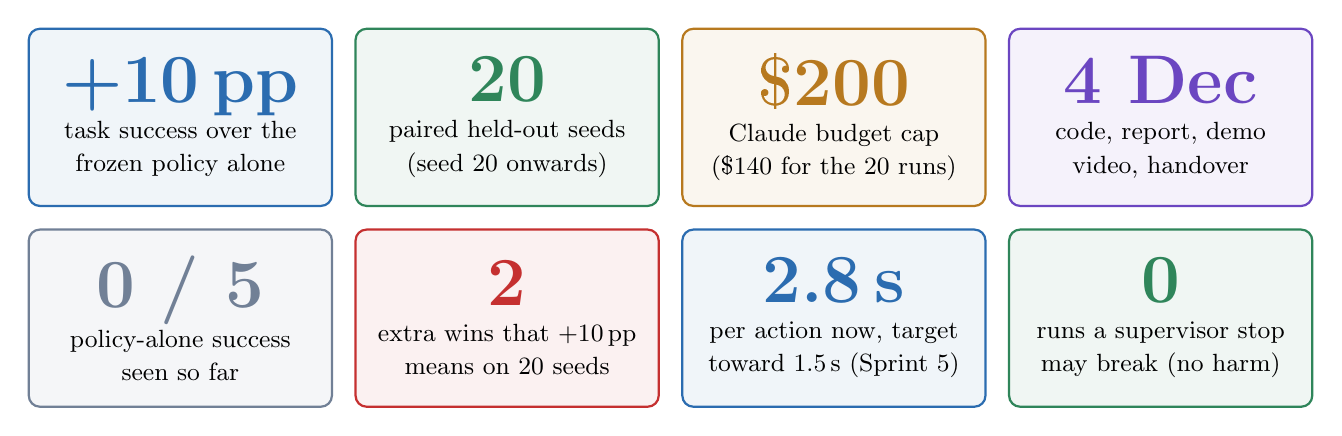
\begin{tikzpicture}[tile/.style={draw=#1,fill=#1!7,rounded corners=4pt,thick,minimum width=3.85cm,minimum height=2.25cm,align=center}]
  \node[tile=sky]   (a) at (0,0)      {\Huge\bfseries\color{sky}+10\,pp\\[1pt]\small task success over the\\\small frozen policy alone};
  \node[tile=leaf]  (b) at (4.15,0)   {\Huge\bfseries\color{leaf}20\\[1pt]\small paired held-out seeds\\\small (seed 20 onwards)};
  \node[tile=sun]   (c) at (8.3,0)    {\Huge\bfseries\color{sun}\$200\\[1pt]\small Claude budget cap\\\small (\$140 for the 20 runs)};
  \node[tile=grape] (d) at (12.45,0)  {\Huge\bfseries\color{grape}4 Dec\\[1pt]\small code, report, demo\\\small video, handover};
  \node[tile=stone] (e) at (0,-2.55)  {\Huge\bfseries\color{stone}0 / 5\\[1pt]\small policy-alone success\\\small seen so far};
  \node[tile=rose]  (f) at (4.15,-2.55) {\Huge\bfseries\color{rose}2\\[1pt]\small extra wins that +10\,pp\\\small means on 20 seeds};
  \node[tile=sky]   (g) at (8.3,-2.55)  {\Huge\bfseries\color{sky}2.8\,s\\[1pt]\small per action now, target\\\small toward 1.5\,s (Sprint 5)};
  \node[tile=leaf]  (h) at (12.45,-2.55){\Huge\bfseries\color{leaf}0\\[1pt]\small runs a supervisor stop\\\small may break (no harm)};
\end{tikzpicture}
\end{center}

\begin{keyidea}
\textbf{The promise:} by 4 December, a supervision harness lifts the success rate of the frozen Neotix
\emph{hanging\_mug} policy by at least 10 percentage points, \textbf{without retraining it}, measured on
20 starting scenes nobody tuned on, with every run's latency and cost reported.\\[3pt]
\textbf{The client's attitude:} \emph{``an honest result will be valuable to us whichever way the numbers land.''}
They care more about a clean, honest evaluation than about a flattering number.
\end{keyidea}

\noindent\textbf{How to read this guide.}
Section~\ref{sec:sow} walks through the SoW itself. Sections~\ref{sec:seeds}--\ref{sec:project} explain seeds
from scratch with a toy example, then show how this project uses them. Section~\ref{sec:asks} lists everything
Birhanu asked for, and Section~\ref{sec:reading} shows what the result can and cannot claim.
Section~\ref{sec:open} lists the decisions we still have to make and where the code on \texttt{main} does not yet
match the SoW. Section~\ref{sec:checklist} is a checklist.

\begin{center}
\begin{tikzpicture}[doc/.style={draw=#1,fill=#1!8,thick,rounded corners=3pt,minimum width=5.4cm,minimum height=1.25cm,align=center,font=\small}]
  \node[doc=sky]  (sow) at (0,0) {\faFileContract\ \textbf{Final SoW} (6 pp.)\\the contract: what, when, how judged};
  \node[doc=grape](mail) at (8.6,0) {\faEnvelope\ \textbf{E-mail thread} (6 messages)\\how the client reads the contract};
  \draw[arr,<->] (sow) -- node[above=2pt,lbl]{edits folded in} (mail);
  \node[lbl,below=2mm of sow]  {signed by Birhanu, 17 Nov};
  \node[lbl,below=2mm of mail] {Sascha's sign-off is an e-mail (23 Nov):\\\textbf{include it with the submission}};
\end{tikzpicture}
\end{center}

\clearpage
% ====================================================================== 1. SoW
\section{What the SoW says}\label{sec:sow}

\subsection{The commitment and the ``Hill''}

The SoW's success statement (its ``Hill'') is written from the engineer's point of view:

\begin{quotebox}{SoW \S1.1 -- the Hill}
Neotix engineers can run a two-arm manipulation task with their existing trained policy and see it complete
tasks more often, at least 10 percentage points more than the policy alone under the same starting conditions,
without having to retrain the policy.
\end{quotebox}

\noindent Every phrase is a testable condition:

\begin{center}
\begin{tabularx}{\linewidth}{@{}>{\bfseries}p{4.6cm}X@{}}
\toprule
Phrase in the Hill & What it forces us to do\\
\midrule
``existing trained policy'' & The Neotix checkpoint \tool{robotwin-hanging-mug-dit} is served \emph{unchanged} on a Modal T4.\\
``complete tasks'' & An episode counts only when RoboTwin's native success check passes \emph{and} a short post-release window confirms the mug stays on the rack.\\
``at least 10 percentage points more'' & Supervised success rate $-$ policy-alone success rate $\ge 0.10$.\\
``under the same starting conditions'' & \textbf{Paired seeds}: both settings face the same scenes (Section~\ref{sec:seeds}).\\
``without having to retrain'' & Supervision lives outside the policy: perception, planner, bounded skills.\\
\bottomrule
\end{tabularx}
\end{center}

\subsection{What changed since the Initial SoW (29 Sep)}

\begin{center}
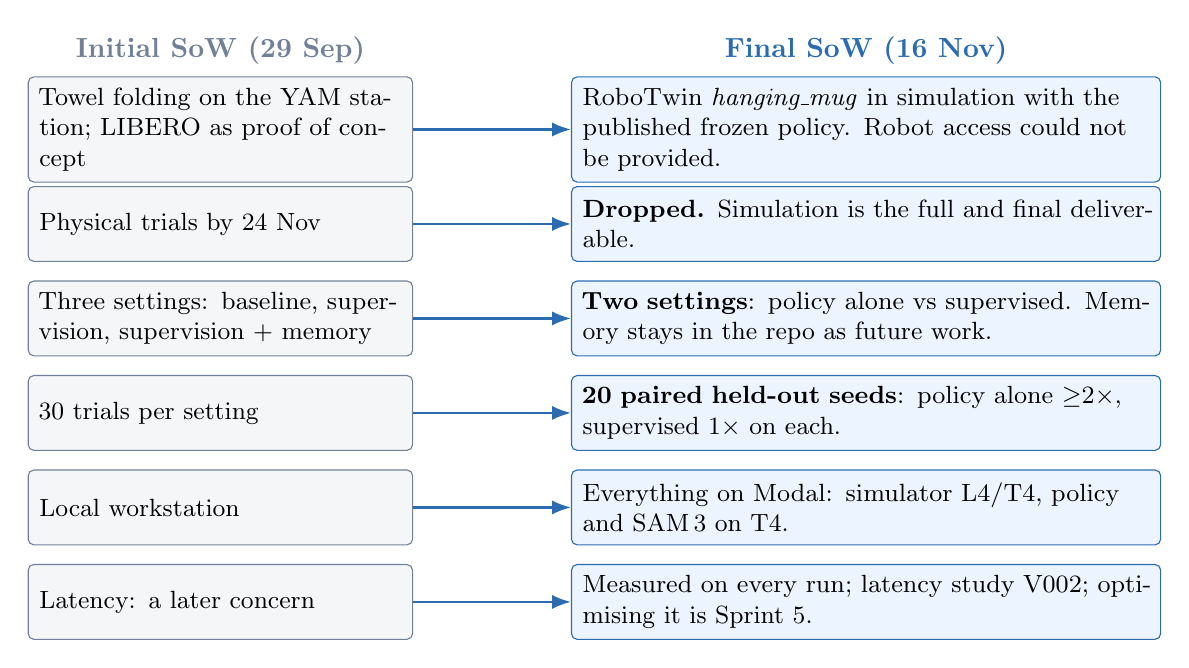
\begin{tikzpicture}[old/.style={draw=stone,fill=stonelight,rounded corners=2pt,text width=4.6cm,align=left,font=\small,inner sep=4pt,minimum height=0.95cm},
                    new/.style={draw=sky,fill=skylight,rounded corners=2pt,text width=7.2cm,align=left,font=\small,inner sep=4pt,minimum height=0.95cm}]
  \node[font=\bfseries\color{stone}] at (0,1.0) {Initial SoW (29 Sep)};
  \node[font=\bfseries\color{sky}] at (8.2,1.0) {Final SoW (16 Nov)};
  \foreach \y/\o/\n in {
     0/{Towel folding on the YAM station; LIBERO as proof of concept}/{RoboTwin \emph{hanging\_mug} in simulation with the published frozen policy. Robot access could not be provided.},
    -1.2/{Physical trials by 24 Nov}/{\textbf{Dropped.} Simulation is the full and final deliverable.},
    -2.4/{Three settings: baseline, supervision, supervision + memory}/{\textbf{Two settings}: policy alone vs supervised. Memory stays in the repo as future work.},
    -3.6/{30 trials per setting}/{\textbf{20 paired held-out seeds}: policy alone $\ge$2$\times$, supervised 1$\times$ on each.},
    -4.8/{Local workstation}/{Everything on Modal: simulator L4/T4, policy and SAM\,3 on T4.},
    -6.0/{Latency: a later concern}/{Measured on every run; latency study V002; optimising it is Sprint 5.}}{
    \node[old] (o) at (0,\y) {\o};
    \node[new] (n) at (8.2,\y) {\n};
    \draw[arr,draw=sky] (o.east) -- (n.west);
  }
\end{tikzpicture}
\end{center}

\subsection{How one supervised episode works}

The supervisor never replaces the policy. The frozen policy does most of the motion through \tool{VLA\_ACT}; the
planner only steps in with a bounded analytic skill when the evidence shows a failure.

\begin{center}
\begin{tikzpicture}[st/.style={box=#1,minimum width=3.3cm,minimum height=1.25cm}]
  \node[st=stone] (obs) at (0,0)     {\faCamera\ \textbf{Observe}\\RGB-D from 3 cameras\\+ 14-DoF robot state};
  \node[st=leaf]  (per) at (4.6,0)   {\faEye\ \textbf{Perceive}\\SAM\,3 masks + depth\\$\to$ 3-D poses, facts};
  \node[st=grape] (dec) at (10.4,0)  {\faBrain\ \textbf{Decide}\\Claude Opus picks\\one checked skill};
  \node[st=sky]   (act) at (10.4,-2.6){\faRobot\ \textbf{Act}\\\tool{VLA\_ACT} (policy chunk)\\or a bounded skill};
  \node[st=sun]   (ver) at (4.6,-2.6){\faClipboardCheck\ \textbf{Verify}\\stop checks, budgets,\\log everything};
  \draw[arr] (obs) -- (per);
  \draw[arr] (per) -- node[below=2pt,lbl]{true / false /\\\emph{unknown}} (dec);
  \draw[arr] (dec) -- (act);
  \draw[arr] (act) -- (ver);
  \draw[arr] (ver.west) -| (obs.south);
  \node[lbl,text width=9cm,anchor=north] at (6.5,-3.6) {Skills: \tool{VLA\_ACT}, \tool{MOVE\_TO}, \tool{ROTATE\_WRIST}, \tool{SET\_GRIPPER}, \tool{RELEASE} (gated by \tool{release\_ready}), \tool{ABORT}.\\No simulator object state ever reaches the planner: only public RGB-D evidence.};
\end{tikzpicture}
\captionof{figure}{The loop each planner turn runs (simplified from SoW Figures 1 and 2).}
\end{center}

\subsection{Requirements at a glance}

\begin{center}\small
\begin{tabularx}{\linewidth}{@{}l X l@{}}
\toprule
ID & Requirement (paraphrased) & Proved by\\
\midrule
\multicolumn{3}{@{}l}{\color{sky}\bfseries User, functional}\\
UF1 & Automatic failure detection and bounded recovery, no routine human help & intervention log\\
UF2 & One command starts a trial; review outcome, video, every decision & \tool{run\_skills.py}\\
UF3 & Compare the same seeds with supervision on and off & \textbf{paired seeds}\\
\multicolumn{3}{@{}l}{\color{sky}\bfseries User, non-functional}\\
UN1 & $\ge$ +10\,pp task success, no policy retraining & headline KPI\\
UN2 & Safe execution in a completion time agreed with the sponsor & latency target 1.5\,s/action\\
UN3 & Evidence that holds on starting positions \emph{not used for tuning} & \textbf{held-out seeds}\\
\multicolumn{3}{@{}l}{\color{sky}\bfseries System, functional}\\
SF1 & Monitor images, state, actions; let the policy act or stop it and run one skill & harness loop\\
SF2 & Task facts (lifted, staged, toppled, near rack, release-ready) from public RGB-D only, \emph{unknown} when unsure & perception\\
SF3 & Log every observation, decision, skill result, timing and cost; replay offline & JSONL traces\\
\multicolumn{3}{@{}l}{\color{sky}\bfseries System, non-functional}\\
SN1 & Precision before recall: a wrong ``true'' is worse than ``unknown''; no simulator state to the planner & predicate scoring\\
SN2 & Bounded skill parameters; gripper opens only when release is judged safe; one GPU job at a time & skill schemas\\
SN3 & Every run records config, commit, seed, model and prompt versions, timings, tokens, cost & manifest\\
SN4 & Per-stage latency (median, P95) for every evaluated run & latency report\\
\bottomrule
\end{tabularx}
\end{center}

\subsection{How success is measured (the KPI table)}

\begin{center}\small
\begin{tabularx}{\linewidth}{@{}>{\bfseries}l X >{\raggedright\arraybackslash}p{3.4cm}@{}}
\toprule
KPI & How it is verified & Target\\
\midrule
Task success & Native checker + post-release window; 95\% Wilson intervals; paired counts (won, lost, tied); per-stage completion (grasp, handoff, hang) & supervised $\ge$ policy alone + 10\,pp\\
Does no harm & Seeds where the policy alone succeeds and supervised fails, with the cause from logs and video & 0 caused by a supervisor stop\\
Perception & Offline scoring of every predicate against simulator labels: precision, recall, unknown rate, false trues & precision $\ge$ 0.95 on \tool{release\_ready}\\
Interventions & Count, type and outcome of each recovery skill, with the evidence that triggered it & all logged and explained\\
Latency, cost & Median and P95 per stage, seconds per action, Claude tokens and dollars per episode & every run; toward 1.5\,s/action\\
Software & CPU test suite on every PR; replay checks for perception changes & 100\% passing\\
\bottomrule
\end{tabularx}
\end{center}

\subsection{Budget, compute and latency}

\begin{center}
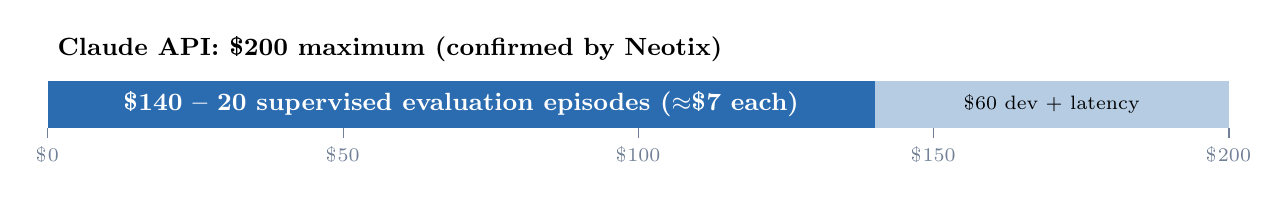
\begin{tikzpicture}[x=0.075cm]
  \node[anchor=west,font=\bfseries\small] at (0,1.0) {Claude API: \$200 maximum (confirmed by Neotix)};
  \fill[sky] (0,0) rectangle (140,0.6);
  \fill[sky!35] (140,0) rectangle (200,0.6);
  \node[white,font=\small\bfseries] at (70,0.3) {\$140 -- 20 supervised evaluation episodes ($\approx$\$7 each)};
  \node[font=\scriptsize] at (170,0.3) {\$60 dev + latency};
  \foreach \v in {0,50,100,150,200}{\draw[stone] (\v,0) -- (\v,-0.12) node[below,font=\scriptsize,text=stone]{\$\v};}
\end{tikzpicture}

\vspace{4mm}
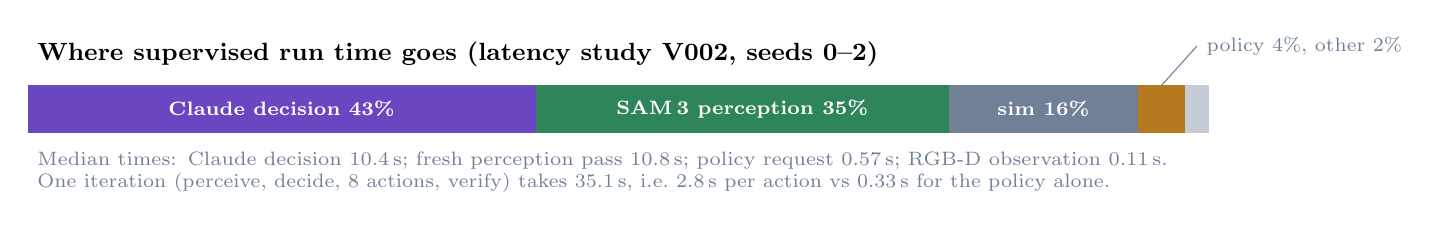
\begin{tikzpicture}[x=0.15cm]
  \node[anchor=west,font=\bfseries\small] at (0,1.0) {Where supervised run time goes (latency study V002, seeds 0--2)};
  \fill[grape]   (0,0) rectangle (43,0.6);  \node[white,font=\scriptsize\bfseries] at (21.5,0.3) {Claude decision 43\%};
  \fill[leaf]    (43,0) rectangle (78,0.6); \node[white,font=\scriptsize\bfseries] at (60.5,0.3) {SAM\,3 perception 35\%};
  \fill[stone]   (78,0) rectangle (94,0.6); \node[white,font=\scriptsize\bfseries] at (86,0.3) {sim 16\%};
  \fill[sun]     (94,0) rectangle (98,0.6);
  \fill[stone!40](98,0) rectangle (100,0.6);
  \draw[stone] (96,0.6) -- (99,1.1) node[right,font=\scriptsize,text=stone]{policy 4\%, other 2\%};
  \node[anchor=west,font=\scriptsize,text=stone,text width=14.5cm] at (0,-0.5)
   {Median times: Claude decision 10.4\,s; fresh perception pass 10.8\,s; policy request 0.57\,s; RGB-D observation 0.11\,s.
    One iteration (perceive, decide, 8 actions, verify) takes 35.1\,s, i.e.\ 2.8\,s per action vs 0.33\,s for the policy alone.};
\end{tikzpicture}
\end{center}

\begin{eli5}
Most of the time goes on \emph{deciding}, not moving. The Sprint 5 job is to cut 2.8\,s per action toward 1.5\,s
without losing success: first the 32/16 inspection schedule, then fewer SAM\,3 prompts and cameras per turn,
one change at a time, re-measured on about 8 of the evaluation seeds.
\end{eli5}

\subsection{Risks the SoW names}

\begin{center}\small
\begin{tabularx}{\linewidth}{@{}l X X@{}}
\toprule
Type & Risk & Mitigation\\
\midrule
\chip{rose}{tech} & Supervision does not beat the policy; a stop ends runs the policy would have finished & Hand back to the policy whenever evidence is missing; report honestly either way\\
\chip{rose}{tech} & Perception blind spots (end-on toppled mug, mug held sideways) give a wrong ``true'' & Precision-first predicates, pose-axis release veto, never open on one fact alone\\
\chip{rose}{tech} & \textbf{Policy not repeatable within a seed} (up to 0.53\,rad difference) & \textbf{Paired seeds, $\ge$20 per setting, intervals, no claim from one run}\\
\chip{rose}{tech} & Latency and cost limit the number of runs & Cost tracked per run; the 20 evaluation episodes funded first\\
\chip{sun}{dep} & Claude rate limits or budget exhausted (happened once) & Serial runs; offline replay and scripted planner for development\\
\chip{sun}{dep} & Modal preemption, capacity, renderer hang & Auto restart; GPU fallback L4$\to$A10G$\to$T4; time limits\\
\chip{grape}{org} & Five open PRs conflict before the freeze & Merge order agreed; one owner per PR; freeze 20 Nov\\
\bottomrule
\end{tabularx}
\end{center}

\clearpage
% ====================================================================== 2. Seeds from scratch
\section{Seeds from scratch}\label{sec:seeds}

\subsection{A seed names one starting scene}

At reset, a simulator draws random numbers to lay out the scene: where the mug is, how it is turned, where the rack
sits. Those numbers come from a \emph{pseudo}-random generator, which only looks random: start it from the same
number and it produces exactly the same sequence. That starting number is the \textbf{seed}.

\begin{center}
\begin{tikzpicture}
  \node[box=sun,minimum width=1.8cm] (s) at (0,0) {\textbf{seed = 7}};
  \node[box=stone,minimum width=2.6cm] (g) at (3.2,0) {pseudo-random\\generator};
  \node[box=stone,minimum width=3.0cm,font=\ttfamily\small] (n) at (7.0,0) {0.83, 0.97, 0.12, ...};
  \node[box=leaf,minimum width=2.6cm] (sc) at (11.6,0) {\faImage\ scene \#7\\mug at (8,\,9)};
  \draw[arr] (s) -- (g); \draw[arr] (g) -- (n); \draw[arr] (n) -- node[above,lbl]{lay out} (sc);
  \draw[arr,draw=sun,dashed] (s.south) to[bend right=12] node[below,lbl,text=sun]{same seed, today or next week $\Rightarrow$ \textbf{identical scene}} (sc.south);
\end{tikzpicture}
\end{center}

\begin{eli5}
A seed is a \emph{name for a starting situation}. ``Seed 7'' means ``the scene you get when the generator starts
from 7''. It fixes the \textbf{problem} posed to the robot, not the \textbf{answer}.
\end{eli5}

\subsection{Toy example: a mug on a 10$\times$10 table}

Suppose reset places the mug in a random cell:
\texttt{rng = random.Random(seed); mug = (rng.randint(0, 9), rng.randint(0, 9))}.

\begin{center}
\begin{tikzpicture}[scale=0.42]
  \fill[stonelight] (0,0) rectangle (10,10);
  \draw[stone!50,step=1] (0,0) grid (10,10);
  \draw[thick,stone] (0,0) rectangle (10,10);
  % robot base at the bottom centre
  \fill[stone] (4,-1.2) rectangle (6,-0.3); \node[font=\scriptsize,text=white] at (5,-0.75) {robot};
  \foreach \x/\y/\s/\c in {2/5/0/leaf,9/0/1/rose,4/4/2/leaf,8/9/7/sun}{
     \fill[\c] (\x+0.5,\y+0.5) circle (0.38);
     \node[font=\tiny\bfseries,text=white] at (\x+0.5,\y+0.5) {\s};
  }
  \foreach \i in {0,...,9}{\node[font=\tiny,text=stone] at (\i+0.5,10.5) {\i}; \node[font=\tiny,text=stone] at (-0.5,\i+0.5) {\i};}
  \node[anchor=west,font=\small] at (11.5,8.5) {\begin{tabular}{@{}cll@{}}
    \toprule seed & mug at & what it is like\\ \midrule
    \textcolor{leaf}{\faCircle}\ 0 & (2,\,5) & middle of the table: easy\\
    \textcolor{rose}{\faCircle}\ 1 & (9,\,0) & far corner: hard to reach\\
    \textcolor{leaf}{\faCircle}\ 2 & (4,\,4) & easy\\
    \textcolor{sun}{\faCircle}\ 7 & (8,\,9) & near the edge\\ \bottomrule\end{tabular}};
  \node[anchor=north west,font=\small,text width=7.2cm] at (11.5,4.6) {Some seeds are easy and some are hard. \textbf{That is
    exactly why seeds matter}: a difference between two systems can come from \emph{which scenes they got} rather
    than from the systems themselves.};
\end{tikzpicture}
\end{center}

\subsection{Use 1 -- a fair comparison: pairing}

To test whether supervision helps, you could give each setting different seeds. But if the policy alone happens
to get the corner mugs, it looks worse for reasons that have nothing to do with supervision. \textbf{Pairing}
removes this: both settings play the \emph{same} seeds, so each seed is a head-to-head match on an identical scene.

\begin{center}
\begin{tikzpicture}[sc/.style={circle,draw=#1,fill=#1!15,thick,minimum size=7mm,inner sep=0,font=\scriptsize\bfseries}]
  \node[font=\bfseries\small,text=rose] at (2.5,1.3) {\faTimes\ Unpaired: different scenes};
  \node[lbl] at (-0.9,0.4) {policy\\alone}; \node[lbl] at (-0.9,-0.6) {super-\\vised};
  \foreach \i/\s/\c in {0/1/rose,1/7/sun,2/1/rose,3/7/sun,4/1/rose}{\node[sc=\c] at (\i*1.2,0.4) {\s};}
  \foreach \i/\s/\c in {0/0/leaf,1/2/leaf,2/0/leaf,3/2/leaf,4/0/leaf}{\node[sc=\c] at (\i*1.2,-0.6) {\s};}
  \node[lbl,text width=5.6cm] at (2.4,-1.6) {supervised got the easy scenes: any gap is partly luck of the draw};
  \begin{scope}[xshift=8.7cm]
  \node[font=\bfseries\small,text=leaf] at (2.5,1.3) {\faCheck\ Paired: same scenes};
  \node[lbl] at (-0.9,0.4) {policy\\alone}; \node[lbl] at (-0.9,-0.6) {super-\\vised};
  \foreach \i/\s/\c in {0/0/leaf,1/1/rose,2/2/leaf,3/7/sun,4/9/stone}{\node[sc=\c] at (\i*1.2,0.4) {\s}; \node[sc=\c] at (\i*1.2,-0.6) {\s};
     \draw[stone,densely dotted] (\i*1.2,0.05) -- (\i*1.2,-0.25);}
  \node[lbl,text width=5.6cm] at (2.4,-1.6) {each column is one match: same scene, only supervision differs};
  \end{scope}
\end{tikzpicture}
\end{center}

\noindent Scoring a paired toy run on five seeds:

\begin{center}
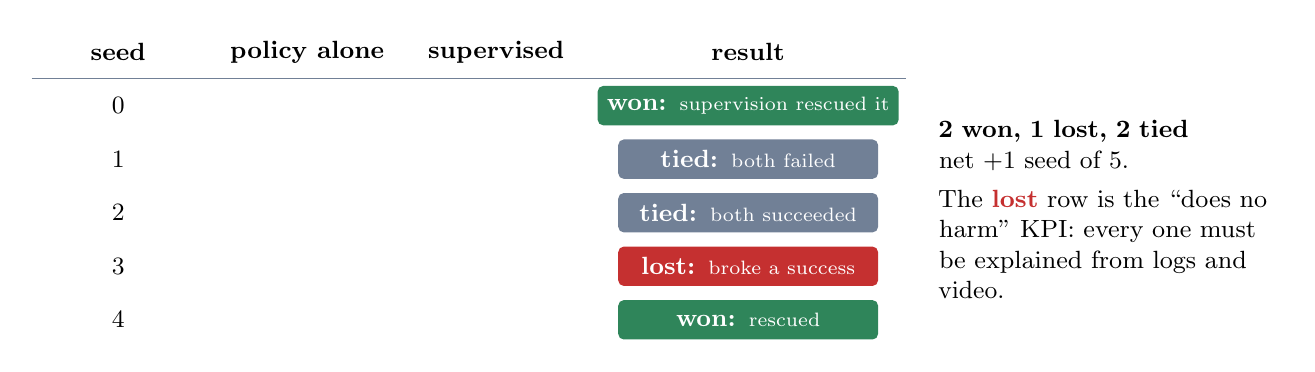
\begin{tikzpicture}[cell/.style={minimum width=2.3cm,minimum height=0.62cm,font=\small},
                    res/.style={rounded corners=2pt,minimum width=3.3cm,minimum height=0.5cm,font=\small\bfseries,text=white}]
  \node[cell,font=\small\bfseries] at (0,0) {seed};
  \node[cell,font=\small\bfseries] at (2.4,0) {policy alone};
  \node[cell,font=\small\bfseries] at (4.8,0) {supervised};
  \node[cell,font=\small\bfseries] at (8.0,0) {result};
  \draw[stone] (-1.1,-0.33) -- (10,-0.33);
  \foreach \y/\s/\a/\b/\r/\c/\t in {
     1/0/\no/\yes/won/leaf/supervision rescued it,
     2/1/\no/\no/tied/stone/both failed,
     3/2/\yes/\yes/tied/stone/both succeeded,
     4/3/\yes/\no/lost/rose/broke a success,
     5/4/\no/\yes/won/leaf/rescued}{
    \node[cell] at (0,-0.68*\y) {\s};
    \node[cell] at (2.4,-0.68*\y) {\a};
    \node[cell] at (4.8,-0.68*\y) {\b};
    \node[res,fill=\c] at (8.0,-0.68*\y) {\r: {\normalfont\scriptsize \t}};
  }
  \node[anchor=west,font=\small,text width=4.3cm] at (10.3,-2.0) {\textbf{2 won, 1 lost, 2 tied}\\net $+1$ seed of 5.\\[3pt]
    The \textcolor{rose}{\textbf{lost}} row is the ``does no harm'' KPI: every one must be explained from logs and video.};
\end{tikzpicture}
\end{center}

\subsection{Use 2 -- honesty: held-out seeds}

While building, we look at failures and tune thresholds, prompts and recovery skills. Suppose we keep tuning until
the far-corner mug (seed~1) works. Some of that tuning may only help \emph{that corner}. Scoring ourselves on seed~1
afterwards is grading ourselves on the exam we studied from.

\begin{center}
\begin{tikzpicture}
  \node[box=sun,minimum width=5.4cm,minimum height=1.9cm] (dev) at (0,0) {\faTools\ \textbf{Development seeds}\\[2pt]look, debug, tune,\\review videos, build memory};
  \node[box=leaf,minimum width=5.4cm,minimum height=1.9cm] (ho) at (8,0) {\faLock\ \textbf{Held-out seeds}\\[2pt]nobody looks until the freeze,\\then scored \textbf{once}};
  \node[box=grape,minimum width=3.0cm] (fr) at (4,-2.4) {\faSnowflake\ \textbf{freeze}\\config, prompts,\\commit, seed list};
  \draw[arr] (dev) |- (fr); \draw[arr] (fr) -| (ho);
  \node[lbl] at (0,1.35) {= the training/practice set};
  \node[lbl] at (8,1.35) {= the test set};
  \node[lbl,text width=4.6cm] at (10.2,-2.4) {The held-out score is the only one that predicts scenes we have never seen (UN3).};
\end{tikzpicture}
\end{center}

\begin{keyidea}
This is the train/test split you know from ML, with the \emph{seed list} as the dataset. Once a held-out seed has been
watched, debugged or tuned on, it is \textbf{contaminated} and becomes a development seed for good.
\end{keyidea}

\subsection{The twist: same seed, different outcome}

A seed fixes the scene, but not everything after it. The Neotix policy is a diffusion-style model (the
\tool{-dit} in its name) that samples its actions, and GPU arithmetic is not bit-exact. Two runs from the identical
scene can drift apart: the SoW records commanded joints differing by \textbf{up to 0.53\,rad within one seed}.

\begin{center}
\begin{tikzpicture}
  \node[box=sun,minimum width=1.8cm] (st) at (0,0) {seed 0\\scene};
  \draw[very thick,sky,-{Latex}] (st.east) .. controls (2.5,0.1) and (4.5,0.4) .. (7.2,1.2) node[right,font=\small,text=leaf] {\faCheck\ mug hung on rack};
  \draw[very thick,sky!45,-{Latex}] (st.east) .. controls (2.5,-0.1) and (4.5,-0.6) .. (7.2,-1.2) node[right,font=\small,text=rose] {\faTimes\ grasp slips};
  \node[lbl] at (2.4,0.6) {run A}; \node[lbl] at (2.4,-0.65) {run B};
  \draw[stone,dashed] (3.6,-0.25) -- (3.6,0.4); \node[lbl] at (3.6,0.75) {paths split};
\end{tikzpicture}
\end{center}

\begin{careful}[Why this matters]
In the toy table, seed~0 might have \emph{failed} with the policy alone today and \emph{succeeded} tomorrow. A ``win''
on that seed could be luck, not supervision. That is why the SoW runs the policy alone \textbf{at least twice} per seed
and never draws a conclusion from a single run.
\end{careful}

% ====================================================================== 3. Seeds in this project
\section{Seeds in this project}\label{sec:project}

One seed is one RoboTwin \emph{hanging\_mug} episode: a specific starting layout of the mug and rack in front of the
two-arm robot. The harness calls \tool{reset(seed)}, then runs up to 900 actions with the same success check in both
settings.

\subsection{The seed map}

\begin{center}
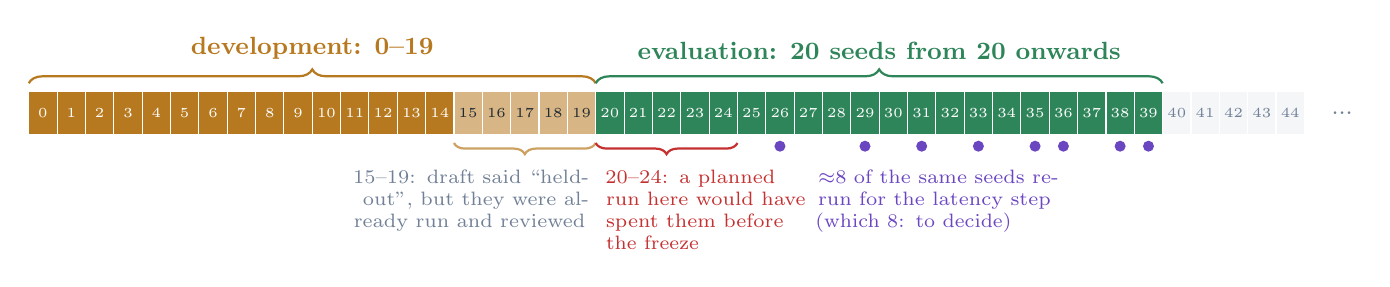
\begin{tikzpicture}[sd/.style={minimum width=0.36cm,minimum height=0.55cm,draw=white,inner sep=0,font=\tiny}]
  \foreach \i in {0,...,14}  {\node[sd,fill=sun,text=white]       at (\i*0.36,0) {\i};}
  \foreach \i in {15,...,19} {\node[sd,fill=sun!55,text=ink,pattern color=sun] at (\i*0.36,0) {\i};}
  \foreach \i in {20,...,39} {\node[sd,fill=leaf,text=white]      at (\i*0.36,0) {\i};}
  \foreach \i in {40,...,44} {\node[sd,fill=stonelight,text=stone] at (\i*0.36,0) {\i};}
  \node[font=\small,text=stone] at (45*0.36+0.3,0) {...};
  % braces
  \draw[decorate,decoration={brace,amplitude=5pt},thick,sun] (-0.18,0.38) -- node[above=5pt,font=\small\bfseries,text=sun]{development: 0--19} (19*0.36+0.18,0.38);
  \draw[decorate,decoration={brace,amplitude=5pt},thick,leaf] (20*0.36-0.18,0.38) -- node[above=5pt,font=\small\bfseries,text=leaf]{evaluation: 20 seeds from 20 onwards} (39*0.36+0.18,0.38);
  \draw[decorate,decoration={brace,amplitude=4pt,mirror},thick,sun!70] (15*0.36-0.18,-0.38) -- node[pos=1,below=6pt,anchor=north east,lbl,text width=3.1cm,align=right]{15--19: draft said ``held-out'', but they were already run and reviewed} (19*0.36+0.18,-0.38);
  \draw[decorate,decoration={brace,amplitude=4pt,mirror},thick,rose] (20*0.36-0.18,-0.38) -- node[pos=0,below=6pt,anchor=north west,lbl,text width=2.6cm,align=left,text=rose]{20--24: a planned run here would have spent them before the freeze} (24*0.36+0.18,-0.38);
  \foreach \i in {26,29,31,33,35,36,38,39} {\fill[grape] (\i*0.36,-0.42) circle (0.07);}
  \node[lbl,text=grape,text width=3.2cm,align=left,anchor=north west] at (27*0.36,-0.6) {$\approx$8 of the same seeds re-run for the latency step (which 8: to decide)};
\end{tikzpicture}
\end{center}

\subsection{What each evaluation seed gets}

\begin{center}
\begin{tikzpicture}[run/.style={minimum width=0.62cm,minimum height=0.48cm,draw=white,inner sep=0}]
  \foreach \j in {0,...,19}{\pgfmathtruncatemacro{\s}{20+\j}\node[font=\tiny,text=stone] at (\j*0.62,0.45) {\s};}
  \foreach \j in {0,...,19}{
     \node[run,fill=stone!70] at (\j*0.62,0) {};
     \node[run,fill=stone!45] at (\j*0.62,-0.5) {};
     \node[run,fill=grape]    at (\j*0.62,-1.0) {};}
  \foreach \j in {6,9,11,13,15,16,18,19}{\node[run,fill=sun] at (\j*0.62,-1.5) {};}
  \node[anchor=east,font=\small] at (-0.45,0)    {policy alone, run 1};
  \node[anchor=east,font=\small] at (-0.45,-0.5) {policy alone, run 2};
  \node[anchor=east,font=\small] at (-0.45,-1.0) {supervised};
  \node[anchor=east,font=\small] at (-0.45,-1.5) {latency re-run};
  \node[lbl] at (5.9,0.85) {evaluation seed};
  \node[anchor=north,font=\scriptsize,text=ink] at (5.9,-1.95) {\textcolor{stone}{\faSquare}\ 40 policy-alone runs, $\approx$5\,min each, \textbf{no Claude cost}\quad
    \textcolor{grape}{\faSquare}\ 20 supervised runs, 35--40\,min, $\approx$\$140\quad
    \textcolor{sun}{\faSquare}\ $\approx$8 latency re-runs};
\end{tikzpicture}
\end{center}

\subsection{How the code keeps held-out seeds clean}

\begin{center}
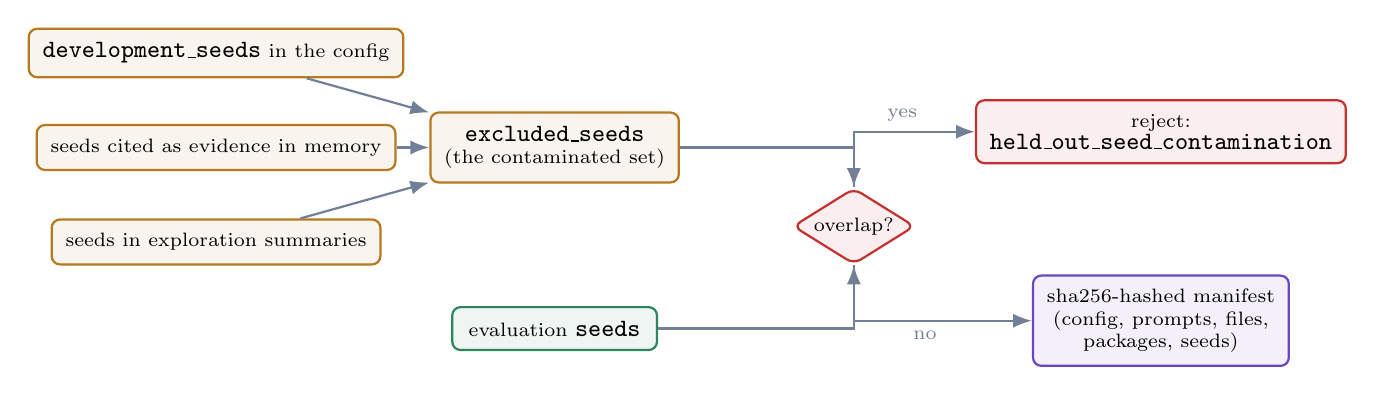
\begin{tikzpicture}[src/.style={box=sun,minimum width=3.6cm,font=\scriptsize},nd/.style={box=#1,font=\scriptsize}]
  \node[src] (a) at (0,1.2)  {\tool{development\_seeds} in the config};
  \node[src] (b) at (0,0)    {seeds cited as evidence in memory};
  \node[src] (c) at (0,-1.2) {seeds in exploration summaries};
  \node[nd=sun,minimum width=2.6cm] (ex) at (4.3,0) {\tool{excluded\_seeds}\\(the contaminated set)};
  \node[nd=leaf,minimum width=2.6cm] (ev) at (4.3,-2.3) {evaluation \tool{seeds}};
  \node[nd=rose,diamond,aspect=1.6,inner sep=1pt] (chk) at (8.1,-1.0) {overlap?};
  \node[nd=rose,minimum width=3.2cm] (bad) at (12,0.2) {reject:\\\tool{held\_out\_seed\_contamination}};
  \node[nd=grape,minimum width=3.2cm] (ok) at (12,-2.2) {sha256-hashed manifest\\(config, prompts, files,\\packages, seeds)};
  \draw[arr] (a) -- (ex); \draw[arr] (b) -- (ex); \draw[arr] (c) -- (ex);
  \draw[arr] (ex) -| (chk); \draw[arr] (ev) -| (chk);
  \draw[arr] (chk) |- node[pos=0.7,above,lbl]{yes} (bad);
  \draw[arr] (chk) |- node[pos=0.7,below,lbl]{no} (ok);
\end{tikzpicture}
\end{center}

\begin{incode}
\tool{harness/evaluation/manifest.py}: \tool{freeze()} builds \tool{excluded\_seeds} from the three sources above;
\tool{FrozenEvaluation.split()} raises \tool{held\_out\_seed\_contamination} on any overlap, and
\tool{EvaluationSettings} already rejects evaluation seeds listed as development seeds. The manifest is hashed, so
\tool{run\_evaluation.py run -{}-sha256 ...} refuses a manifest that was edited after the freeze, and \tool{verify()}
refuses to run if the code has drifted (\tool{frozen\_runtime\_changed}). See Section~\ref{sec:open} for where the
code on \texttt{main} still differs from the SoW.
\end{incode}

\subsection{What the SoW commits to about seeds}

\begin{center}\small
\begin{tabularx}{\linewidth}{@{}>{\bfseries}l X@{}}
\toprule
Where in the SoW & What it says\\
\midrule
Hill (\S1.1) & Success is ``measured on \textbf{20 paired held-out seeds}''.\\
Changes table & ``20 paired held-out seeds: the policy alone \textbf{at least twice} and supervised \textbf{once} on each.''\\
\S3.1 & ``Seeds \textbf{0--19 are development seeds}; the evaluation uses seeds from \textbf{20 onwards}, untouched until the freeze.'' \tool{run\_evaluation.py} ``rejects seeds that were used for tuning''. Same 900-action limit and success check for every run.\\
KPI table & Paired counts (won, lost, tied), 95\% Wilson intervals, per-stage completion (grasp, handoff, hang).\\
UN3 & ``Evidence that holds on starting positions not used for tuning'': the reason held-out seeds exist.\\
Risk table & Policy not repeatable within a seed $\to$ paired seeds, $\ge$20 per setting, intervals, no single-run claims.\\
\S3.2 & The latency step re-runs about 8 of the evaluation seeds.\\
Table 4 & By 20 Nov: freeze config, prompts and commit and \textbf{send Neotix the held-out seed list}.\\
\bottomrule
\end{tabularx}
\end{center}

% ====================================================================== 4. Asks
\section{What Birhanu asked of us}\label{sec:asks}

Birhanu's reply of 17 Nov accepted the SoW (\emph{``the work is strong''}) and then set the rules for the frozen
evaluation. He stressed that none of them change our scope. Most were folded into the final SoW; the rest are
expectations for the runs and the report.

\begin{quotebox}{What he praised}
One-command supervised episode; perception built only on public RGB-D with mug-base error down to 2--3\,mm; 696
passing tests; an honest latency study. Moving to \emph{hanging\_mug} in simulation ``was the right call''. The failure
review (8 of 9 failures happen before the hang) ``is exactly the analysis we hoped to see'', and moving recovery work
upstream to the grasp and handoff ``is the right priority''.
\end{quotebox}

\subsection{About seeds and the baseline}

\begin{ask}{1}{Treat seeds 0--19 as development}
\textbf{He said:} the draft listed 0--14 as development, but the progress update showed 15--19 were also evaluated and
reviewed. ``Leave 20 onwards untouched until the freeze.'' The planned run on seeds 20--24 ``should use development
seeds instead, otherwise those five can no longer count as held-out.''\\[2pt]
\textbf{Why:} a seed you have watched is contaminated, like a test question you have already seen.
\end{ask}

\begin{ask}{2}{Run the policy alone at least twice on every evaluation seed}
\textbf{He said:} policy-alone episodes take about five minutes and need no Claude calls, so run them at least twice.
``That separates the gain from supervision from the policy's own run-to-run variation, which you already flagged.''\\[2pt]
\textbf{Why:} the same seed can give a different outcome (Section~\ref{sec:seeds}). Two baseline runs show how much the
policy varies by itself, so that variation is not credited to supervision. It is cheap, so there is no reason not to.
\end{ask}

\begin{ask}{3}{State the baseline and report paired counts}
\textbf{He said:} state the policy-alone success rate in the report (0 of 5 so far). ``With a baseline near zero,
+10 points on 20 seeds is two extra successes.'' Report the paired counts (won, lost, tied) next to the intervals.\\[2pt]
\textbf{Why:} two successes is a small number; the raw paired counts let the reader judge it (Section~\ref{sec:reading}).
\end{ask}

\begin{ask}{4}{Per-stage completion for both settings}
\textbf{He said:} add per-stage completion (grasp, handoff, hang) for both settings, ``so progress is visible even where
the full task does not complete.''\\[2pt]
\textbf{Why:} if the full hang is rare, the stages still show where supervision moved the episode forward.
\end{ask}

\subsection{About budget, evidence, latency and integration}

\begin{ask}{5}{Claude budget: \$200 maximum, evaluation first}
At about \$7 per supervised episode, \$200 covers about 28 episodes. Protect the 20 evaluation episodes first (\$140).
The remaining \$60 covers development and the latency step on about 8 of the same seeds. Offline replay and the scripted
planner cost nothing in Claude calls and are the way to develop before the freeze. 20 paired seeds is the right size for
this budget. (The draft SoW said about \$300; the final says \$200.)
\end{ask}

\begin{ask}{6}{Public evidence only}
The progress update mentions development-oracle checks that remain in grasp recovery. \textbf{Any that still exist at the
freeze must be listed in the evaluation manifest}, because the SoW promises that no simulator state reaches the planner.
Apply the same success check, including the post-release window, to both settings.
\end{ask}

\begin{ask}{7}{Latency target}
The SoW left the completion time ``to be agreed''. His suggestion, now in the SoW: move from 2.8 toward about
\textbf{1.5 seconds per action, with no loss of success}, on the seeds re-run in Sprint 5.
\end{ask}

\begin{ask}{8}{Integration}
Five PRs were open (203, 204, 206, 207, 208), some stacked. Agree the merge order now and include the latency study,
because the SoW cites its numbers.
\end{ask}

\begin{ask}{9}{The final report}
Add one short section, written from our simulation evidence alone, on what would have to change before this could run
on real hardware: \textbf{asynchronous decisions, real depth noise, safety limits}. Add a note on the \textbf{memory design as
future work}. No physical trials are expected.
\end{ask}

\subsection{The five small edits (all done in the signed SoW)}

\begin{center}\small
\begin{tabularx}{\linewidth}{@{}c X@{}}
\toprule
& Edit\\
\midrule
\yes & Development seed range reads 0--19\\
\yes & Resources table: Claude maximum \$200, evaluation at 20 paired seeds\\
\yes & One project name everywhere: ``Agent-Aware'' (the draft said ``Agent-Augmented'')\\
\yes & Typo in \S2.2 (``being are tracked'')\\
\yes & Optional YAM demonstration removed: simulation is the full and final deliverable; nothing depends on hardware\\
\bottomrule
\end{tabularx}
\end{center}

\subsection{The timeline he set}

\begin{center}
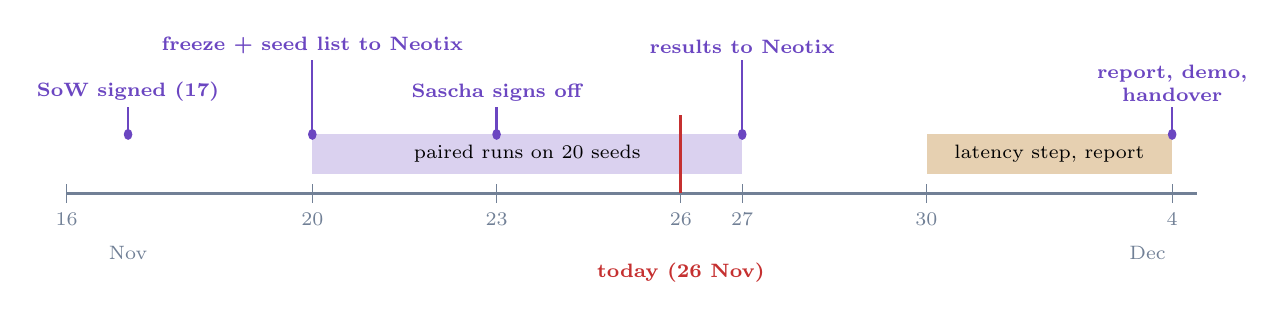
\begin{tikzpicture}[x=0.78cm]
  % days 16 Nov (0) .. 4 Dec (18)
  \draw[thick,stone] (0,0) -- (18.4,0);
  \foreach \d/\l in {0/16,4/20,7/23,10/26,11/27,14/30,18/4}{\draw[stone] (\d,0.12) -- (\d,-0.12) node[below,font=\scriptsize,text=stone]{\l};}
  \node[font=\scriptsize,text=stone] at (1,-0.75) {Nov}; \node[font=\scriptsize,text=stone] at (17.6,-0.75) {Dec};
  \fill[grape!25] (4,0.25) rectangle (11,0.75); \node[font=\scriptsize] at (7.5,0.5) {paired runs on 20 seeds};
  \fill[sun!35] (14,0.25) rectangle (18,0.75); \node[font=\scriptsize] at (16,0.5) {latency step, report};
  \foreach \d/\t/\h in {1/{SoW signed (17)}/1.25,4/{freeze + seed list to Neotix}/1.85,7/{Sascha signs off}/1.25,11/{results to Neotix}/1.85,18/{report, demo,\\handover}/1.25}{
     \draw[grape,thick] (\d,0.75) -- (\d,\h-0.15); \fill[grape] (\d,0.75) circle (0.07);
     \node[font=\scriptsize\bfseries,text=grape,align=center,anchor=south] at (\d,\h-0.2) {\t};}
  \draw[rose,very thick] (10,0) -- (10,1.0); \node[font=\scriptsize\bfseries,text=rose] at (10,-1.0) {today (26 Nov)};
\end{tikzpicture}
\end{center}

\begin{careful}[Sending the seed list first is deliberate]
Sending the held-out seed list to Neotix \emph{before} running is a commitment device: it shows we did not pick seeds
after seeing outcomes. The same logic applies to every analysis choice in Section~\ref{sec:open}: fix it before the
numbers come in.
\end{careful}

\clearpage
% ====================================================================== 5. Reading the result
\section{What the result can and cannot claim}\label{sec:reading}

\subsection{+10 points on 20 seeds is two seeds}

With 20 seeds, each seed is worth 5 percentage points. Starting from a baseline near 0\%, the target is reached by
\textbf{two} extra successes.

\begin{center}
\begin{tikzpicture}[sq/.style={minimum size=0.55cm,draw=white,thick,inner sep=0}]
  \node[anchor=east,font=\small] at (-0.3,0) {policy alone (0/20)};
  \node[anchor=east,font=\small] at (-0.3,-0.7) {supervised (2/20)};
  \foreach \i in {0,...,19}{\node[sq,fill=stone!30] at (\i*0.58,0) {};}
  \foreach \i in {0,...,19}{\node[sq,fill=stone!30] at (\i*0.58,-0.7) {};}
  \foreach \i in {0,1}{\node[sq,fill=leaf] at (\i*0.58,-0.7) {\color{white}\scriptsize\faCheck};}
  \draw[decorate,decoration={brace,amplitude=4pt,mirror},thick,leaf] (-0.27,-1.05) -- node[below=4pt,font=\scriptsize,text=leaf]{+10\,pp} (0.58+0.27,-1.05);
  \node[anchor=west,font=\scriptsize,text=stone] at (3.0,-1.35) {each square is one seed = 5 percentage points};
\end{tikzpicture}
\end{center}

\subsection{Why the intervals and paired counts both matter}

A 95\% Wilson interval shows the range of true success rates consistent with what we saw. With only 20 seeds the
intervals are wide and overlap even when supervision clearly helps on some seeds:

\begin{center}
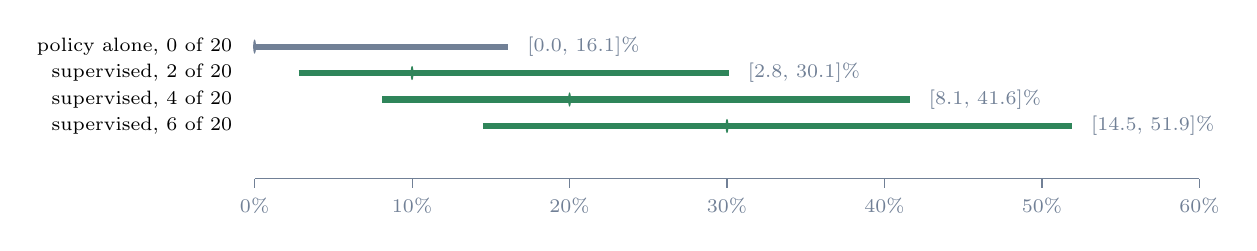
\begin{tikzpicture}[x=0.2cm]
  \draw[stone] (0,0) -- (60,0);
  \foreach \v in {0,10,20,30,40,50,60}{\draw[stone] (\v,0) -- (\v,-0.12) node[below,font=\scriptsize,text=stone]{\v\%};}
  \foreach \y/\k/\lo/\hi/\c/\lab in {
     4.0/0/0.0/16.1/stone/{policy alone, 0 of 20},
     3.2/2/2.8/30.1/leaf/{supervised, 2 of 20},
     2.4/4/8.1/41.6/leaf/{supervised, 4 of 20},
     1.6/6/14.5/51.9/leaf/{supervised, 6 of 20}}{
    \draw[\c,line width=2.2pt] (\lo,\y*0.42) -- (\hi,\y*0.42);
    \fill[\c] (\k*5,\y*0.42) circle (0.09);
    \node[anchor=east,font=\scriptsize] at (-0.8,\y*0.42) {\lab};
    \node[anchor=west,font=\scriptsize,text=stone] at (\hi+0.6,\y*0.42) {[\lo, \hi]\%};
  }
\end{tikzpicture}
\captionof{figure}{95\% Wilson intervals for 20 seeds (computed for this guide). Dots are the observed rate.}
\end{center}

\noindent Pairing adds power the two separate intervals do not show: the question becomes ``on the seeds where the two
settings \emph{disagreed}, how often did supervision win?'' Ties carry no information. A sign test on the disagreeing
seeds gives a feel for how lopsided the split must be before chance becomes an unlikely explanation:

\begin{center}\small
\begin{tabular}{@{}lcccccccc@{}}
\toprule
won / lost on disagreeing seeds & 2/0 & 3/0 & 4/0 & 5/0 & 6/0 & 5/1 & 7/1 & 8/1\\
two-sided sign-test $p$ & 0.50 & 0.25 & 0.13 & 0.06 & \textbf{0.03} & 0.22 & 0.07 & \textbf{0.04}\\
\bottomrule
\end{tabular}
\end{center}

\begin{keyidea}
Hitting +10\,pp (2 extra wins) meets the \emph{contract}, but it is not statistically convincing on its own. That is
fine: the SoW promises the target, and Birhanu asked for the paired counts, intervals and per-stage completion so that the
reader can judge the size of the effect honestly. Report all of them, including every \textbf{lost} seed with its cause.
\end{keyidea}

\subsection{Per-stage completion}

The task has three stages. Reporting how far each run got shows progress even when the full hang fails, and shows
\emph{where} supervision helps.

\begin{center}
\begin{tikzpicture}
  \foreach \i/\s/\c in {0/grasp/sky,1/handoff/grape,2/hang/leaf}{
    \node[box=\c,minimum width=2.6cm,minimum height=0.9cm] (s\i) at (\i*3.6,0) {\textbf{\s}};}
  \draw[arr] (s0) -- (s1); \draw[arr] (s1) -- (s2);
  \node[box=leaf,minimum width=2.6cm,minimum height=0.9cm] (ok) at (10.8,0) {\faCheck\ success\\{\scriptsize native check + post-release}};
  \draw[arr] (s2) -- (ok);
  \node[lbl,text width=6.6cm] at (3.6,-1.1) {The failure review found 8 of 9 failures happen \emph{before} the hang, which is why recovery work moved upstream to grasp and handoff.};
\end{tikzpicture}
\end{center}

% ====================================================================== 6. Open decisions and gaps
\section{Open decisions and gaps to close}\label{sec:open}

\subsection{Decision: how to pair two baseline runs with one supervised run}

The SoW and the e-mail ask for the policy alone twice and supervised once per seed, but neither defines how to score
the pair when the two baseline runs disagree. Two reasonable rules:

\begin{center}
\begin{tikzpicture}[opt/.style={box=#1,text width=6.6cm,align=left,minimum height=3.0cm,anchor=north}]
  \node[opt=sky] (a) at (0,0) {\textbf{A. Seed-level, strict}\\[2pt]
    A seed is a baseline success if \emph{either} policy-alone run succeeded. Then score won/lost/tied against the one
    supervised run.\\[3pt]
    \textcolor{leaf}{\faPlus} harder for supervision to ``win''; conservative.\\
    \textcolor{rose}{\faMinus} one lucky baseline run hides a real gain.};
  \node[opt=grape] (b) at (7.4,0) {\textbf{B. Run-level rate, seed-level pairing}\\[2pt]
    Baseline rate = successes over all 40 policy-alone runs. Each seed's baseline score is 0, 0.5 or 1, compared with
    the supervised 0 or 1.\\[3pt]
    \textcolor{leaf}{\faPlus} uses all the data; shows variation directly.\\
    \textcolor{rose}{\faMinus} ``half wins'' are harder to explain.};
\end{tikzpicture}
\end{center}

\begin{careful}[Decide before the numbers come in]
Pick one rule, write it down, and ideally record it in the evaluation manifest or README \emph{before} looking at the
results. Choosing after seeing the numbers looks like choosing the rule that flatters them. Whatever we pick, also show
the raw table (seed, run 1, run 2, supervised) so the reader can apply the other rule.
\end{careful}

\subsection{Where \texttt{main} does not yet match the SoW}

Checked on \texttt{main} at commit \tool{9bdba29} (26 Nov). Some of this may already be handled on a branch or on
someone's machine; if so, it still needs to land before results go to Neotix.

\begin{center}\small
\begin{tabularx}{\linewidth}{@{}>{\raggedright\arraybackslash}p{4.3cm} >{\raggedright\arraybackslash}X >{\raggedright\arraybackslash}p{3.4cm}@{}}
\toprule
Where & What it does now & What the SoW / Birhanu need\\
\midrule
\tool{configs/\allowbreak evaluation.yaml} & \tool{seeds: [1001, 1002]}, \tool{development\_seeds: [0, 1, 2, 3]}, scripted planner, condition \tool{oracle\_assisted\_acquisition}; the settings model rejects any handoff configuration & dev 0--19, 20 seeds from 20 onwards, Claude planner, full task\\
\tool{development/hanging/\allowbreak seed\_evaluation.py} (the paired runner used for the 5-seed study) & One \tool{policy\_only} and one \tool{supervised} run per seed. Its \tool{attempts=2} retries a \emph{crashed} launch; it is not a second baseline run. No check that seeds avoid 0--19 (its own example uses 15--19). Report has no Wilson intervals or won/lost/tied & 2 baseline runs per seed; seed guard; paired counts, intervals, per-stage completion\\
\tool{run\_evaluation.py run} & Refuses to run without \tool{-{}-development-oracle} & Ask 6: list every oracle check left at the freeze in the manifest\\
\bottomrule
\end{tabularx}
\end{center}

\begin{incode}
The contamination guard in \tool{harness/evaluation/manifest.py} only protects runs launched through
\tool{run\_evaluation.py}. If the 20-seed evaluation is launched through \tool{seed\_evaluation.py} instead, then
either route it through a frozen manifest or add the same guards there, so that the SoW's sentence ``\tool{run\_evaluation.py}
rejects seeds that were used for tuning'' is true of the runs we actually report.
\end{incode}

% ====================================================================== 7. Checklist
\section{Checklist}\label{sec:checklist}

\begin{center}\small
\begin{tabularx}{\linewidth}{@{}c X >{\raggedright\arraybackslash}p{3.3cm}@{}}
\toprule
& Item & Source\\
\midrule
\multicolumn{3}{@{}l}{\color{sky}\bfseries Before and during the evaluation runs}\\
$\square$ & Agree and write down the pairing rule (Section~\ref{sec:open}) & SoW KPI table\\
$\square$ & Freeze config, prompts and commit; evaluation seeds all $\ge$ 20 and never looked at & SoW \S3.1, Ask 1\\
$\square$ & Send Neotix the held-out seed list & SoW Table 4\\
$\square$ & List every development-oracle check still present in the manifest & Ask 6\\
$\square$ & Policy alone $\ge$2$\times$ and supervised 1$\times$ on each of 20 seeds, 900-action limit, same success check with post-release window & SoW, Asks 2 and 6\\
$\square$ & Latency and cost logged on every run & SN4, KPI table\\
$\square$ & Keep Claude spend inside \$200, evaluation episodes first; develop on replay and the scripted planner & Ask 5\\
\multicolumn{3}{@{}l}{\color{sky}\bfseries Results to Neotix (27 Nov)}\\
$\square$ & Baseline rate stated; paired won/lost/tied; 95\% Wilson intervals; per-stage completion for both settings & Asks 3 and 4\\
$\square$ & Every lost seed explained from logs and video (``does no harm'') & KPI table\\
$\square$ & Perception precision, recall, unknown rate and false trues; \tool{release\_ready} precision $\ge$ 0.95 & KPI table\\
\multicolumn{3}{@{}l}{\color{sky}\bfseries Sprint 5 and handover (30 Nov -- 4 Dec)}\\
$\square$ & One latency change at a time on $\approx$8 of the same seeds, toward 1.5\,s/action with no loss of success & Ask 7, SoW \S3.2\\
$\square$ & Final report: success rate, latency, cost; real-hardware section; memory as future work & Ask 9\\
$\square$ & Demo video, presentation, reproducible handover package on GitHub & SoW \S3.1\\
$\square$ & E-mail the report to Birhanu, copy Sascha; submit on Canvas with Sascha's sign-off e-mail & SoW \S3.1, 23 Nov e-mail\\
\bottomrule
\end{tabularx}
\end{center}

\vfill
\begin{center}\small\color{stone}
Sources: \emph{Final Statement of Work} (signed 17 Nov 2026) and the e-mail thread ``Neotix Capstone: Progress Report
and Final Statement of Work'' (16--23 Nov 2026). The toy example, interval figure and sign-test table are added
for explanation; the code notes reflect \texttt{main} at \tool{9bdba29}.
\end{center}

\end{document}
